%!TEX root = ../main.tex

\section{Hash chain}

Assume that $H$ is a secure hash function that maps a struct to a 256-bit.

\begin{definition}
A \textbf{hash-chain} is a data-structure composed of nodes called blocks. 
Every block $b$ contains a pointer $b.prev$ to a preceding bock and a field $b.h_{-1}$ 
that contains the hash of the block referenced by $b.prev$.
A block also contains a data item $b.data$.

\begin{itemize}
	\item The hash of a block $b$ is computed as $H(b)= H(b.h_{-1} || b.data)$.
	\item $b.h_{-1}=H(b.prev)$
	\item There exist one block $b_0$, for which $b.prev$ is empty.
	\item For to block $b$ and $b'$, if $b.prev=b'$ we say that $b$ is a \emph{successor} of $b'$.
	
\end{itemize}

In a \textbf{hash-chain} every block has at most one successor.
\end{definition}

\begin{figure}[ht]
	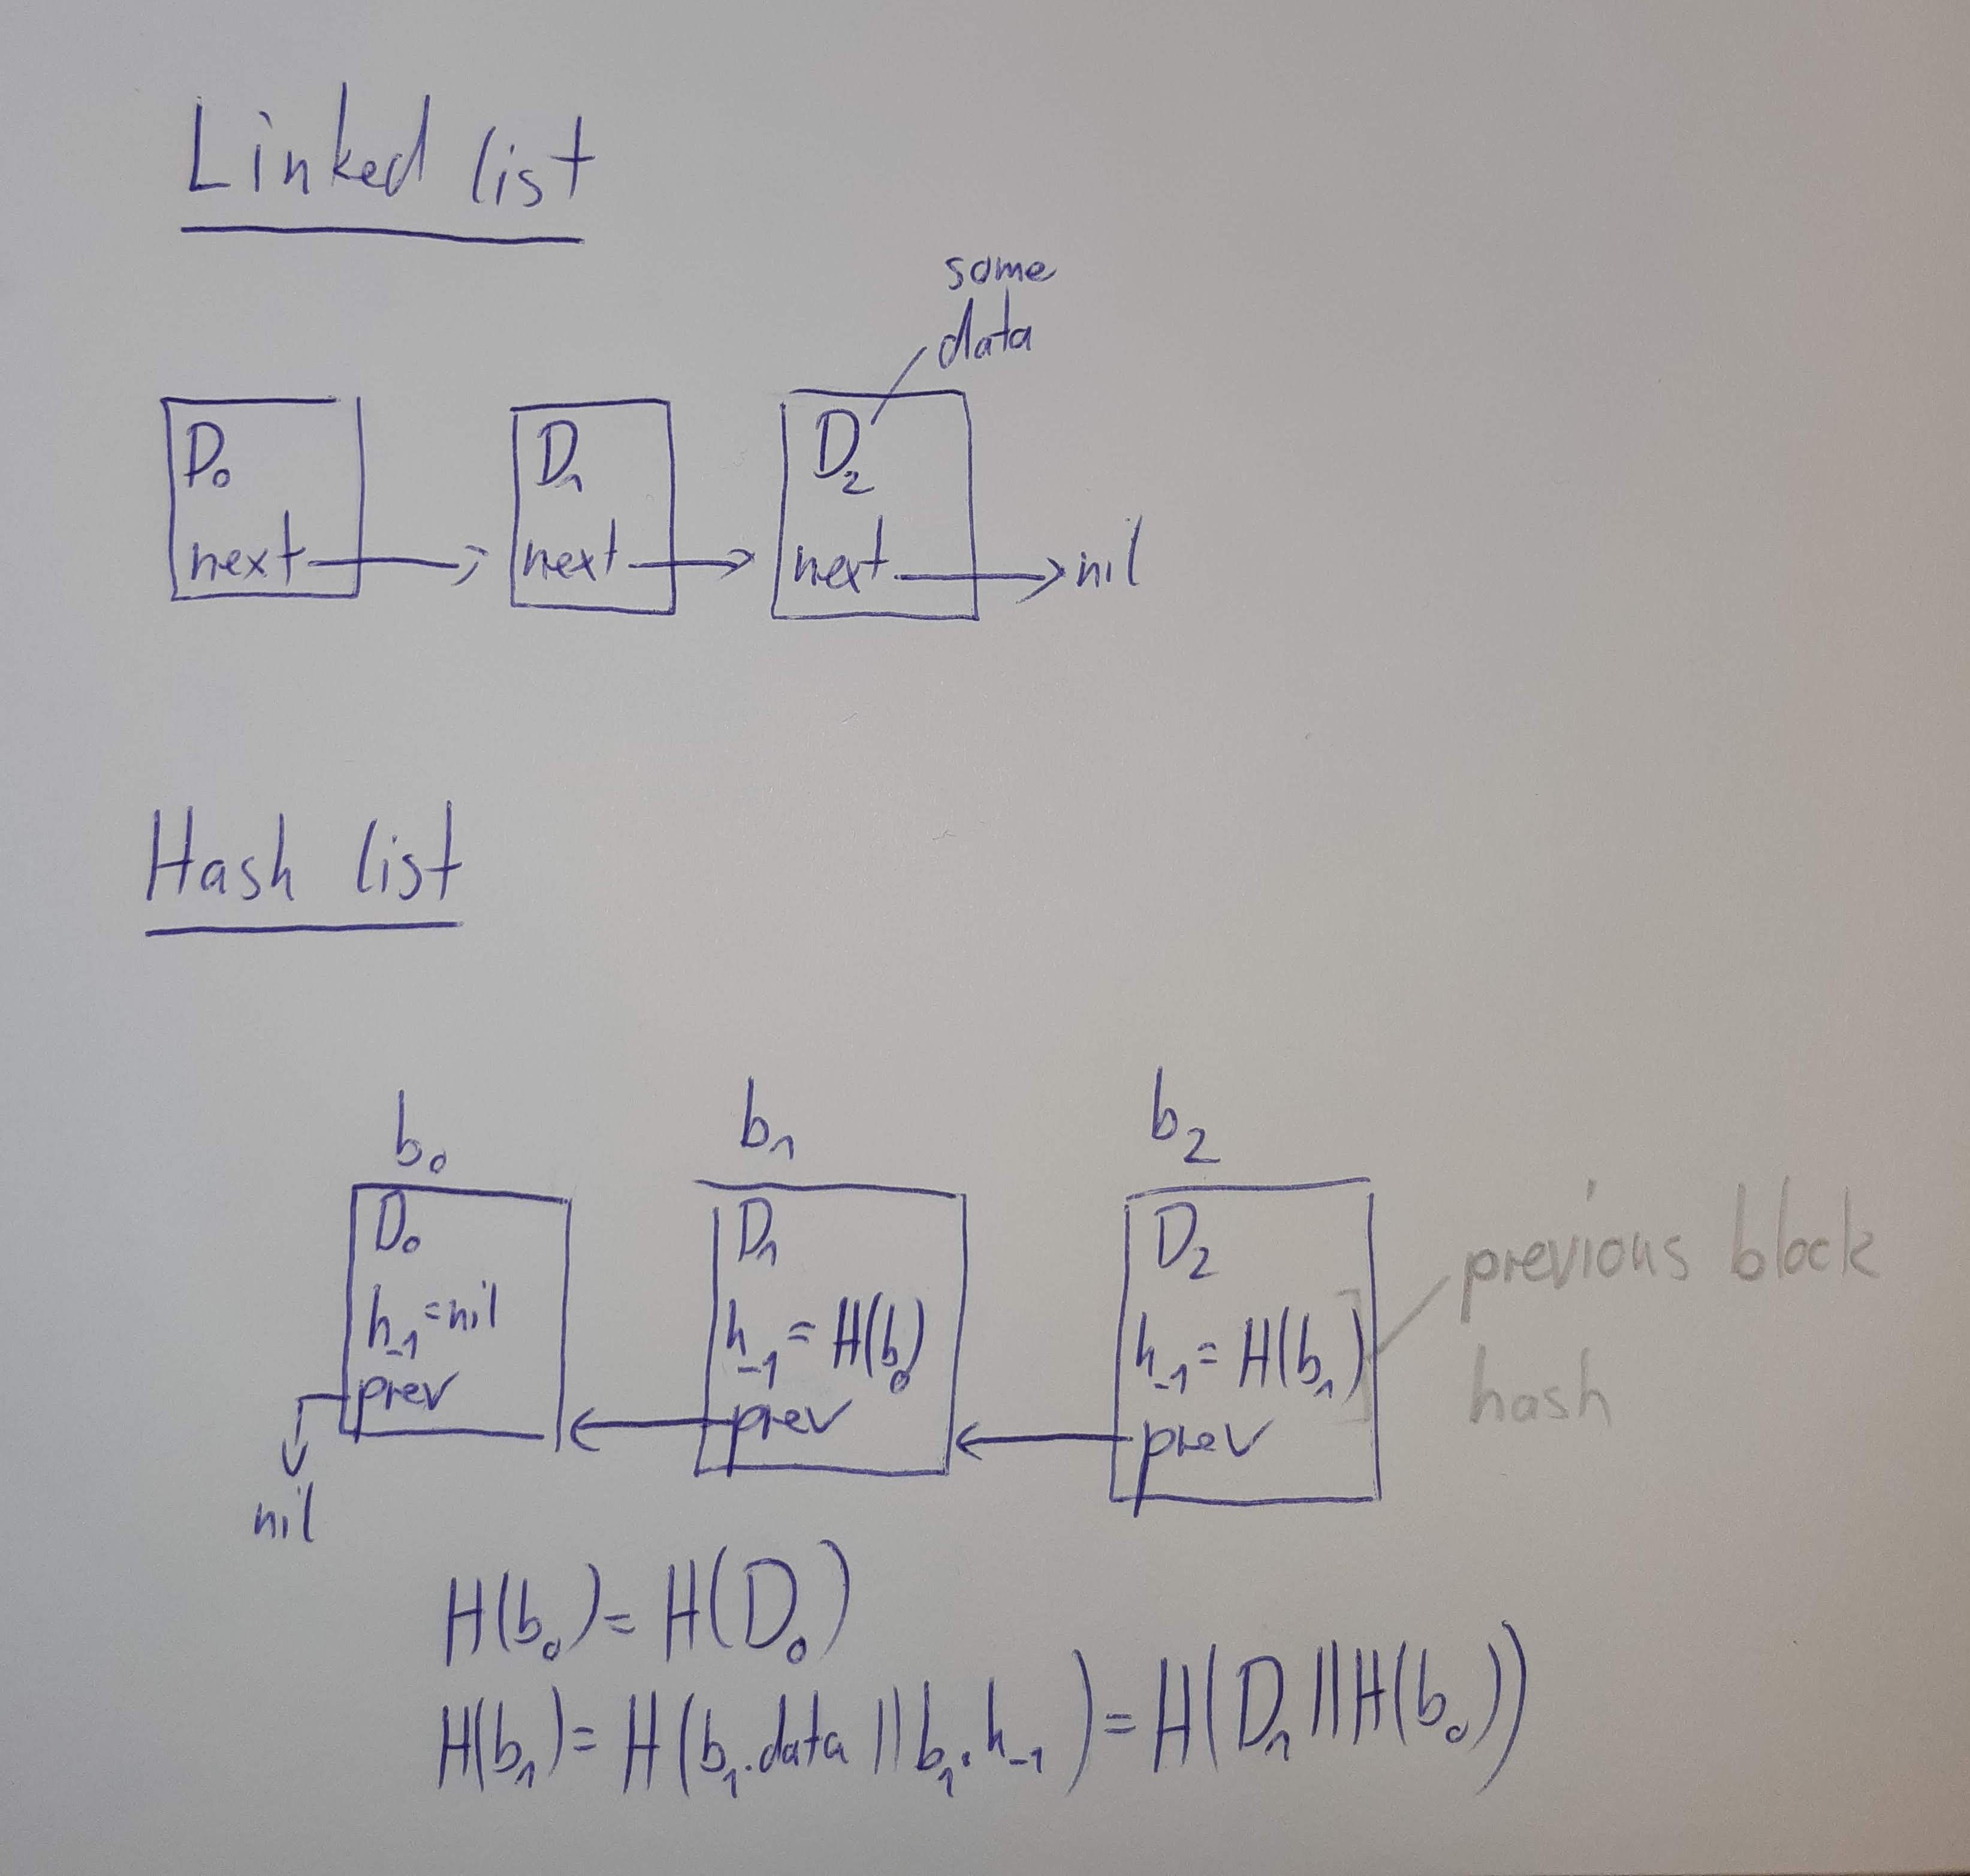
\includegraphics[width=\textwidth]{fig/hash-chain}
	
\end{figure}

\comment{Image}



\begin{lem}
The blocks in a hash-chain can be linearly ordered according to the successor relation with the block $b_0$ as the first block.
\end{lem}


\begin{note}
	If blocks $b_0$, $b_1$ and $b_2$ contain data $D_0$, $D_1$ and $D_2$ then
\begin{align*}
	H(b_0) & = H(D_0)\\
	H(b_1) & = H( H(b_0) || D_1) = H( H(D_0)|| D_1) \\
	H(b_2) & = H( H(b_1) || D_2) = H( H( H(b_0) || D_1)|| D_2) \\
\end{align*}

\end{note}

\question{What happens if we:
\begin{itemize}
	\item Insert a block?
	\item Change the data?
	\item Append a block?
\end{itemize}
}

\question{Given a hash chain $b_0, b_1, b_2, ..., b_n$ which of the following is infeasible.
\begin{itemize}
	\item Create an alternative hash chain $b'_0, b_1, b'_2, ... ,b'_n$ 
	such that $b'_i=b_i$ for $i<3$ and $b'_3 \neq b_3$.
	\item Create an alternative hash chain $b'_0, b_1, b'_2, ... ,b'_n$ such that $b'_n=b_n$ and $b'_1 \neq b_1$.
	\item Create an alternative hash chain $b'_0, b_1, b'_2$ such that $b'_2=b_1$.
	\item Create an alternative hash chain $b'_0, b_1, b'_2, ... ,b'_n, b'_{n+1}$ such that $b'_{n+1}=b_n$.
	\item Assume $n$ is very large, but no $b_i$ has $b_i.data = "hello world"$.
	Create $b'$, s.t., for some $i\leq n$ $H(b')=H(b_i)$ and $b'.data="hello world"$
\end{itemize}
Why?}

\begin{example}
Assume a notary maintains, a hash-chain of all documents it has signed. 
\begin{itemize}
	\item This allows document holders to proof that their document was signed.
	\item This allows to document holders to proof which document was signed first.
	\item Prevent the notary itself to change in which order documents where signed or remove single documents.
\end{itemize}
\end{example}
\question{How can we publish this hash chain?}
\question{What if the notary has very many documents. Can we avoid to have only one document per block? 
Ideas:
\begin{itemize}
	\item Publish multiple hashes?
	\item Hash multiple documents?
\end{itemize}}